% Bản thảo. Mọi con số là macro sinh bởi scripts/make_paper.py (paper/generated/numbers.tex); không gõ tay số vào đây.
% Dựng: python scripts/make_paper.py && cd paper && tectonic main.tex     (hoặc latexmk -pdf main.tex nếu có elsarticle)
\documentclass[preprint,12pt]{elsarticle}
\usepackage{amsmath,amssymb}
\usepackage{booktabs,multirow,graphicx}
\usepackage[table]{xcolor}
\usepackage[hidelinks]{hyperref}
\newcommand{\todo}[1]{\textcolor{red}{[TBD: #1]}}
\newcommand{\draftnote}[1]{\par\noindent\textcolor{blue}{\emph{Draft note: #1}}\par}
% \input ngay trước \bottomrule gây lỗi "Misplaced \noalign"; dùng lệnh nguyên thủy cho thân bảng
\makeatletter\newcommand{\tabinput}[1]{\@@input #1.tex }\makeatother
% Sinh bởi scripts/make_paper.py. KHÔNG sửa tay: chạy lại script khi có kết quả mới.
\newcommand{\AllQHighBelow}{0}
\newcommand{\AmiCleanGainMax}{2.55}
\newcommand{\AmiCleanGainMin}{2.03}
\newcommand{\AmiOnlyVsPubEarvn}{$-$0.51}
\newcommand{\AmiQHighGainMax}{0.35}
\newcommand{\AmiQHighGainMin}{0.18}
\newcommand{\AmiQLowGapMax}{0.53}
\newcommand{\AmiQLowGapMin}{0.40}
\newcommand{\AmiQLowSig}{16}
\newcommand{\AmiQMidGapMax}{0.36}
\newcommand{\AmiQMidGapMin}{0.22}
\newcommand{\AwexMQLowSig}{16}
\newcommand{\AwexSQLowSig}{16}
\newcommand{\BicCleanPsnr}{36.73}
\newcommand{\BicQLowLpips}{0.396}
\newcommand{\BicQLowPsnr}{34.36}
\newcommand{\BlurHi}{0.6}
\newcommand{\BlurLo}{0.2}
\newcommand{\BsrganQLowGap}{1.98}
\newcommand{\BsrganQLowLpips}{0.173}
\newcommand{\CollapseBic}{32.33}
\newcommand{\CollapseBroken}{82}
\newcommand{\CollapsePsnr}{22.08}
\newcommand{\CollapsePub}{36.39}
\newcommand{\DegEffMax}{1.89}
\newcommand{\DegEffMin}{1.30}
\newcommand{\DispEstVsBicMax}{1.96}
\newcommand{\DispEstVsBicMin}{1.12}
\newcommand{\DispEstVsGenMax}{2.40}
\newcommand{\DispEstVsGenMin}{1.49}
\newcommand{\EarvnQLowBelow}{14}
\newcommand{\EarvnQLowSig}{6}
\newcommand{\EstLpipsVsBicMax}{0.146}
\newcommand{\EstLpipsVsBicMin}{0.116}
\newcommand{\EstLpipsVsGenMax}{0.046}
\newcommand{\EstLpipsVsGenMin}{0.038}
\newcommand{\EstLpipsVsPubMax}{0.110}
\newcommand{\EstLpipsVsPubMin}{0.049}
\newcommand{\EstVsBicAmiL}{1.13}
\newcommand{\EstVsBicAmiM}{1.45}
\newcommand{\EstVsBicAmiS}{1.81}
\newcommand{\EstVsBicMax}{2.22}
\newcommand{\EstVsBicMin}{1.23}
\newcommand{\EstVsBicQHighMax}{2.30}
\newcommand{\EstVsBicQHighMin}{0.99}
\newcommand{\EstVsBicQLowMax}{1.87}
\newcommand{\EstVsBicQLowMin}{1.01}
\newcommand{\EstVsGenFoldMax}{1.17}
\newcommand{\EstVsGenFoldMin}{0.96}
\newcommand{\EstVsGenMax}{2.09}
\newcommand{\EstVsGenMin}{1.08}
\newcommand{\EstVsJpgHighMax}{0.58}
\newcommand{\EstVsJpgHighMin}{0.41}
\newcommand{\EstVsJpgLowMax}{0.14}
\newcommand{\EstVsJpgLowMin}{0.06}
\newcommand{\EstVsJpgMax}{0.26}
\newcommand{\EstVsJpgMin}{0.14}
\newcommand{\EstVsMixMax}{\todo{n2c}}
\newcommand{\EstVsMixMin}{\todo{n2c}}
\newcommand{\EstVsMixOnMixMax}{\todo{n2c}}
\newcommand{\EstVsMixOnMixMin}{\todo{n2c}}
\newcommand{\EstVsPubCleanMax}{1.77}
\newcommand{\EstVsPubCleanMin}{1.21}
\newcommand{\EstVsPubMax}{1.89}
\newcommand{\EstVsPubMin}{1.32}
\newcommand{\EstVsUniMax}{\todo{n2c}}
\newcommand{\EstVsUniMin}{\todo{n2c}}
\newcommand{\ExtraAmi}{$-$0.02}
\newcommand{\ExtraAwexM}{$+$0.19}
\newcommand{\ExtraAwexS}{$+$0.30}
\newcommand{\ExtraEarvn}{$+$0.62}
\newcommand{\FitLarge}{81}
\newcommand{\FitSmall}{621}
\newcommand{\GenVsBicCleanMax}{2.19}
\newcommand{\GenVsBicCleanMin}{0.37}
\newcommand{\GenVsBicEstMax}{$+$0.72}
\newcommand{\GenVsBicEstMin}{$-$0.86}
\newcommand{\JpgEffMax}{2.03}
\newcommand{\JpgEffMin}{1.37}
\newcommand{\LatBsrgan}{13.6}
\newcommand{\LatDisp}{0.34}
\newcommand{\LatRatio}{27}
\newcommand{\LatSpan}{0.50}
\newcommand{\LpipsQLowBetter}{16}
\newcommand{\MixVsUniMax}{\todo{n2c}}
\newcommand{\MixVsUniMin}{\todo{n2c}}
\newcommand{\NAmiAllImg}{700}
\newcommand{\NAmiImg}{420}
\newcommand{\NAmiSubj}{60}
\newcommand{\NAwexMImg}{60}
\newcommand{\NAwexMSubj}{49}
\newcommand{\NAwexSImg}{217}
\newcommand{\NAwexSSubj}{138}
\newcommand{\NEarvnImg}{158}
\newcommand{\NEarvnSubj}{24}
\newcommand{\NFolds}{3}
\newcommand{\NPub}{16}
\newcommand{\NRuns}{30}
\newcommand{\NRunsStable}{30}
\newcommand{\NoiseHi}{6.27}
\newcommand{\NoiseLo}{0.85}
\newcommand{\ParamsRatio}{39}
\newcommand{\ParamsRrdb}{16.7}
\newcommand{\ParamsSpan}{0.43}
\newcommand{\PubVsBicEstMax}{0.59}
\newcommand{\PubVsBicEstMin}{$-$0.43}
\newcommand{\QHighShare}{44.1}
\newcommand{\QLowShare}{51.7}
\newcommand{\RealBic}{80.1}
\newcommand{\RealEst}{58.5}
\newcommand{\RealGen}{78.0}
\newcommand{\RealJpg}{56.7}
\newcommand{\RealTestSubj}{4}
\newcommand{\RealTrainSubj}{8}
\newcommand{\RecEnrolled}{\todo{recog}}
\newcommand{\RecEstVsBic}{\todo{recog}}
\newcommand{\RecEstVsPub}{\todo{recog}}
\newcommand{\RecGallery}{\todo{recog}}
\newcommand{\RecProbes}{\todo{recog}}
\newcommand{\RecRankBic}{\todo{recog}}
\newcommand{\RecRankBsrgan}{\todo{recog}}
\newcommand{\RecRankEst}{\todo{recog}}
\newcommand{\RecRankGen}{\todo{recog}}
\newcommand{\RecRankPub}{\todo{recog}}
\newcommand{\RecRankRef}{\todo{recog}}
\newcommand{\RecSubj}{\todo{recog}}
\newcommand{\RecTrainImg}{\todo{recog}}
\newcommand{\RecTrainSubj}{\todo{recog}}
\newcommand{\RoleAll}{164}
\newcommand{\RoleClf}{16}
\newcommand{\RoleFit}{16}
\newcommand{\RoleTest}{41}
\newcommand{\RoleTrain}{74}
\newcommand{\RoleViewer}{17}
\newcommand{\RrdbVsSpanCleanL}{$+$0.14}
\newcommand{\RrdbVsSpanCleanM}{$+$0.23}
\newcommand{\RrdbVsSpanCleanS}{$+$0.49}
\newcommand{\RrdbVsSpanQLowL}{$-$0.03}
\newcommand{\RrdbVsSpanQLowM}{$-$0.04}
\newcommand{\RrdbVsSpanQLowS}{$-$0.05}
\newcommand{\SpanCleanGainL}{1.84}
\newcommand{\SpanCleanGainM}{2.32}
\newcommand{\SpanCleanGainS}{2.73}
\newcommand{\SpanCleanPsnr}{39.04}
\newcommand{\SpanQLowGapL}{0.42}
\newcommand{\SpanQLowGapM}{0.43}
\newcommand{\SpanQLowGapS}{0.32}
\newcommand{\SpanQLowLpips}{0.358}
\newcommand{\SpanQLowPsnr}{33.93}
\newcommand{\SpreadClean}{0.52}
\newcommand{\SpreadQLow}{0.12}
\newcommand{\StressMaxDrop}{0.85}
\newcommand{\TauRank}{0.03}
\newcommand{\WildCleanGainMax}{4.45}
\newcommand{\WildCleanGainMin}{2.18}
\newcommand{\WildEstGainMax}{$+$0.61}
\newcommand{\WildEstGainMin}{$-$0.25}

\setlength{\belowcaptionskip}{4pt}
\journal{Image and Vision Computing}
\begin{document}
\begin{frontmatter}
\title{Real-Time Super-Resolution for Low-Resolution Ear Images:\\ Degradation Matters More Than Architecture}
% Đơn vị của Thai Le Quang: tạm ghi cùng đơn vị với đồng tác giả; SỬA nếu khác. Tên khoa chưa điền.
\author[hcmou]{Thai Le Quang}
\author[hcmou]{Vinh Truong Hoang\corref{cor1}}
\ead{vinh.th@ou.edu.vn}
\cortext[cor1]{Corresponding author.}
\affiliation[hcmou]{organization={Ho Chi Minh City Open University}, city={Ho Chi Minh City}, country={Vietnam}}
\begin{abstract}
Ear images captured in unconstrained settings are small and JPEG-compressed, whereas efficient super-resolution (SR) networks are designed and ranked on large natural images that are downsampled bicubically and never compressed. We measure what this mismatch costs and where it should be repaired. On a benchmark of ear images with clean ground truth at three input sizes (24 to 48 pixels) and on two in-the-wild ear datasets, the \NPub{} fidelity-oriented SR networks with public weights that we evaluate, including the NTIRE 2026 efficient-SR baseline and five of its entries, lose their advantage over bicubic interpolation once the input is compressed: at JPEG quality 75 all of them fall below bicubic on the controlled benchmark (by \AmiQLowGapMin{} to \AmiQLowGapMax{}~dB), while at quality 93 all of them are above it again. Real small ear images sit on both sides of this threshold. Under compression the \NPub{} architectures differ by only \SpreadQLow{}~dB and a \ParamsRatio{}$\times$ larger network is no better, whereas changing the training degradation of a single backbone changes its PSNR by \DegEffMin{} to \DegEffMax{}~dB. We therefore repair the degradation rather than the architecture: we fine-tune an off-the-shelf real-time network with a compression-aware degradation measured from real small ear images, using a photometric augmentation and in-the-wild ear images without which fine-tuning on laboratory data collapses on bright inputs. On synthesised inputs from three datasets the resulting model exceeds bicubic interpolation by \EstVsBicMin{} to \EstVsBicMax{}~dB, the published weights by \EstVsPubMin{} to \EstVsPubMax{}~dB and a generic real-world degradation pipeline by \EstVsGenMin{} to \EstVsGenMax{}~dB, at an unchanged cost of \LatSpan{}~ms per image on a desktop GPU. On real small ear images that are JPEG-compressed, for which no ground truth exists, rank-1 identification rises from \RecRankBic{}\% with bicubic upscaling and \RecRankPub{}\% with the published weights to \RecRankEst{}\%, and the published weights help only where the files are lightly compressed; on a second dataset whose images carry no compression structure, no upscaling method changes identification. An ablation shows that covering the range of compression levels accounts for the gain; the measured noise and blur do not add to it.

\end{abstract}
\begin{keyword}
ear biometrics \sep image super-resolution \sep efficient super-resolution \sep degradation modelling \sep JPEG compression \sep benchmark
\end{keyword}
\end{frontmatter}

\section{Introduction}
\label{sec:intro}

The ear is a useful biometric trait in surveillance and forensic settings because it can be photographed at a distance and without the cooperation of the subject~\cite{emersic2017ear}. In such footage the ear often occupies a few dozen pixels. In EarVN1.0~\cite{hoang2019earvn}, a collection of ear crops gathered from the web, several thousand images have a short side of 24 to 48 pixels, and all of them are stored with lossy compression. Low resolution and compression are both known to affect ear recognition~\cite{emersic2019uerc,rathgeb2016compression}. An operator who inspects such an image, or a pipeline that requires a larger input, has to enlarge it first, and in interactive or video applications this has to be done in real time.

Efficient single-image super-resolution (SR) is a natural candidate for this step. Work on efficient SR, in recent years organised around the NTIRE Efficient SR challenges~\cite{ren2024ntire,ren2025ntire,ren2026ntire}, has produced networks with a few hundred thousand parameters that run in milliseconds. These networks are designed and ranked under a single protocol: large natural images, bicubic downsampling by a factor of four, and no compression. JPEG-compressed inputs of a few dozen pixels differ from this protocol in content, size and degradation. The one study of SR for ear images that we found~\cite{markicevic2023ear} trains two general-purpose networks and evaluates recognition; it does not address efficient models. It is therefore unclear whether a published efficient SR model is useful on small ear images, and, if it is not, whether the architecture or the training data should be changed.

It is known that SR models trained with bicubic downsampling lose accuracy on compressed inputs~\cite{lugmayr2019unsupervised,chen2018cisrdcnn}, and training with compression is an established remedy~\cite{zhang2021bsrgan,wang2021realesrgan}. This paper does not revisit that general result. It addresses three questions that, to our knowledge, have not been examined for small images of a biometric trait. The first is at which compression level published efficient models stop improving on interpolation, and what determines this level. The second is whether the effect can be observed on real small images, for which no ground truth exists. The third is what is required to adapt a published real-time model to such inputs.

For the first question, we build a benchmark of ear images with clean ground truth at three input sizes from the AMI database, add two in-the-wild datasets, EarVN1.0 and AWEx, and evaluate \NPub{} fidelity-oriented SR networks with public weights, with a control on natural images. In each of the \RatioCells{} settings we tested (four datasets, inputs of \RatioPxMin{} to \RatioPxMax{} pixels, JPEG quality 60 to 93), each model reduces the interpolation error (to \ReduceMin{} to \ReduceMax{} of its value) and amplifies the error added by compression (by a factor of \AmpMin{} to \AmpMax{}). The models fall below bicubic interpolation when the second error exceeds a fraction of the first that lies between \CrossAllMin{} and \CrossAllMax{}, depending on the dataset, and input size has little influence on this point (Section~\ref{sec:natural}). Ear images are smooth and their interpolation error is small. Consistent with this, the gain changes sign at JPEG quality \CrossQAmiMin{} to \CrossQAmiMax{} on AMI, compared with \CrossQNatMin{} to \CrossQNatMax{} on natural images. The two quality levels that account for \QLowShare{}\% and \QHighShare{}\% of the real small ear images we examined, 75 and 93, lie on opposite sides of this point: at quality 75 all \NPub{} models are \AmiQLowGapMin{} to \AmiQLowGapMax{}~dB below bicubic interpolation on AMI, and at quality 93 all of them remain above it (Section~\ref{sec:analysis}).

For the second question, we use two properties of real image files that do not require ground truth: the JPEG quality stored in each file, and the identity label. On the real small images of EarVN1.0, the published SPAN weights change the rank-1 identification rate by \RecQLowPub{} percentage points relative to bicubic upscaling for probes stored at quality 70 to 80, and by \RecQHighPub{} points for probes stored at quality 90 or above, which is consistent with the results on synthesised inputs. A model trained with compression changes it by \RecQLowEst{} and \RecQHighEst{} points. Over all probes the rate is \RecRankBic{}\% with bicubic upscaling, \RecRankPub{}\% with the published weights and \RecRankEst{}\% with the model trained with compression, and a second recogniser gives the same ordering. On AWEx no upscaling method changes the rate significantly. AWEx differs from EarVN1.0 in two respects: its small images show no JPEG block structure, and the recognisers lose much less accuracy between large and small images. We examined these differences after obtaining the result, and the two datasets do not allow them to be separated. We report them as possible conditions for an improvement (Section~\ref{sec:recog}).

For the third question, we compare the effect of the architecture with that of the training degradation. Under JPEG compression at quality 75 the \NPub{} architectures span \SpreadQLow{}~dB, compared with \SpreadClean{}~dB on clean inputs, and a network with \ParamsRatio{} times more parameters does not perform better than a \ParamsSpan{}M-parameter network. Changing the degradation used to fine-tune one backbone changes its PSNR on such inputs by \DegEffMin{} to \DegEffMax{}~dB. We therefore keep a published real-time backbone and change its training. We measure the degradation of real small ear images (the JPEG quality from the quantisation tables stored in the files, the noise level with a standard estimator, and a mild blur selected to match sharpness statistics), and an ablation indicates that the range of JPEG quality levels is the component that matters most. We also report that a model fine-tuned on laboratory images alone fails on bright in-the-wild images (\CollapsePsnr{}~dB, compared with \CollapsePub{}~dB for the weights it was initialised from), and describe two measures that prevented this in our experiments (Section~\ref{sec:stable}).

\paragraph{Contributions}
\begin{enumerate}
\item An evaluation of \NPub{} published efficient SR models on a benchmark of small ear images (clean ground truth at three input sizes, subject-wise cross-validation, two in-the-wild datasets), with a control on natural images. The evaluation relates the advantage of these models over interpolation to the ratio of compression error to interpolation error, and shows that the gain changes sign at a lighter compression for ear images than for natural images.
\item An evaluation on real small ear images without ground truth, based on the JPEG quality stored in the image files and on identity labels, with two datasets and two recognisers. On EarVN1.0 the results agree with those on synthesised inputs. On AWEx no upscaling method changes identification, and we report two differences between the datasets as possible explanations.
\item A training procedure for adapting a published real-time model without architectural changes: a degradation measured from real small ear images, an ablation of its components, and two measures that kept fine-tuning stable on in-the-wild data. The resulting model improves on bicubic interpolation by \EstVsBicMin{} to \EstVsBicMax{}~dB and on the published weights by \EstVsPubMin{} to \EstVsPubMax{}~dB on three datasets.
\end{enumerate}

We do not propose a new architecture. The results have several limits, which we discuss in Section~\ref{sec:discussion}. The model is \EstVsPubCleanMin{} to \EstVsPubCleanMax{}~dB below the published weights on uncompressed inputs. Large perceptual models have a lower LPIPS and a statistically similar identification rate, with a fidelity below bicubic interpolation and \LatRatio{} times the latency on a desktop GPU. The gain is associated with covering the range of compression levels: variants trained with JPEG compression alone give results on real images that we could not distinguish from those of the full measured degradation (Sections~\ref{sec:ablation} and~\ref{sec:recog}).

\section{Related work}
\label{sec:related}
\draftnote{the works in this section were located by web search on 7 October 2026 and are described from their abstracts; none has been read in full. A systematic search of IEEE Xplore and Scopus, and the full text of~\cite{markicevic2023ear}, are still required before the statements marked below can stand.}

\paragraph{Efficient super-resolution} Since SRCNN~\cite{dong2016srcnn}, SR networks have grown from a few layers to deep residual and transformer models~\cite{lim2017edsr,ledig2017srgan,liang2021swinir}. A parallel line of work reduces cost under a fixed quality target, with the NTIRE Efficient SR challenges as its reference benchmark~\cite{ren2024ntire,ren2025ntire,ren2026ntire}; RLFN~\cite{kong2022rlfn}, SAFMN~\cite{sun2023safmn}, SMFANet~\cite{zheng2024smfanet} and SPAN~\cite{wan2024span} are representative, and SPAN serves as the challenge baseline. Real-time SR on mobile hardware has its own benchmark series~\cite{ignatov2021mobile}. All of these models are trained and ranked on DIV2K-style data~\cite{agustsson2017div2k} with bicubic downsampling of large natural images. We take their published weights as they are and ask how they behave on a domain, an input size and a degradation the protocol does not cover.

\paragraph{Real-world degradation} That models trained on bicubic downsampling degrade on real images is well established~\cite{lugmayr2019unsupervised}, and has motivated real paired data~\cite{cai2019realsr}, kernel and noise estimation from real images~\cite{bellkligler2019kernelgan,ji2020realsr}, and broad synthetic pipelines that randomise blur, noise, resizing and JPEG compression~\cite{zhang2021bsrgan,wang2021realesrgan}. The latter are usually combined with adversarial training and target perceptual quality on natural images. The quality of the training images themselves also matters: Ohtani et al.~\cite{ohtani2024rethinking} report that training data with few compression artefacts yield better SR models. Closest to our use of real images of a biometric trait is the work of Bulat et al.~\cite{bulat2018learn}, who learn the degradation of real low-resolution faces with a generative network and then train SR on its outputs. Our approach is deliberately simpler, reading the compression level from the files, and our ablation shows that at inputs of 24 to 48 pixels nothing beyond the range of compression levels needs to be estimated.

\paragraph{Super-resolution of compressed images} Joint compression-artefact reduction and SR has been studied for natural images~\cite{dong2015arcnn,jiang2021fbcnn,chen2018cisrdcnn}, has been the subject of a challenge~\cite{yang2022aim}, and has been addressed with efficient networks for streaming content~\cite{ma2024senn}. That SR of compressed inputs requires compression-aware training is therefore not new, and we do not claim it. What we have not found in this literature is a measurement of where published efficient SR models stop being better than interpolation as compression increases, at input sizes of a few dozen pixels, with a check on real images of the target domain \todo{confirm after a systematic search}.

\paragraph{Low resolution and compression in ear recognition} Image resolution is a recognised source of performance variability in unconstrained ear recognition: it is one of the covariates analysed in the Unconstrained Ear Recognition Challenges~\cite{emersic2017uerc,emersic2019uerc}, and Rathgeb et al.~\cite{rathgeb2016compression} study the effect of image compression on ear recognition systems. These studies measure the effect on recognition; they do not ask what an upscaling step does to the image.

\paragraph{Super-resolution for ears and other biometric traits} SR has a long history in face, iris and other biometric modalities~\cite{nguyen2018srbiometrics}. For faces, the benefit of SR for recognising real low-resolution images has been examined directly~\cite{li2019lowres,menezes2021analysis}. For ears, the only study we found is that of Markičević et al.~\cite{markicevic2023ear}, who train EDSR and SwinIR at $\times2$ and $\times4$ on the UERC data and report rank-1 recognition with a ResNet on the super-resolved images, with original and bicubically interpolated images as baselines \todo{state their degradation model and whether compression is considered, after reading the full text}. We differ in the question asked (which published efficient models work on small compressed ear images, and what must change for them to work), in the evaluation (clean ground truth at three sizes, three datasets, paired statistics by subject, and identification on real small images with subjects disjoint from all training), and in the constraint of real-time inference.

\section{Benchmark}
\label{sec:benchmark}

\subsection{Datasets}
\paragraph{AMI (controlled, clean ground truth)} The AMI ear database~\cite{gonzalez2008ami} contains \NAmiAllImg{} images of 100 subjects, seven per subject, taken indoors at $492\times702$ pixels. Because the originals are large and lightly compressed, downsizing them yields clean ground truth at any small size. We build ground truth at three sizes, with a short side of 96, 144 and 192 pixels; at $\times4$ the inputs then have a short side of 24, 36 and 48 pixels, which is the range in which real small ear images fall. The 36-pixel input is our main cell. Subjects are divided into five folds; in each fold 70 subjects are used for training, 10 for validation and model selection, and 20 for testing, so that every subject is tested exactly once. Two of the five folds were held out during the whole development of this work: every design choice was made on the other three, and the held-out folds were trained and evaluated once, with the configuration frozen, for the results reported here.

\paragraph{EarVN1.0 (in the wild)} EarVN1.0~\cite{hoang2019earvn} contains ear crops of \RoleAll{} subjects collected from the web, with widely varying size, pose and illumination. We assign each subject one role, fixed before any experiment: \RoleTrain{} subjects supply additional training images, \RoleTest{} are used for testing, \RoleFit{} for measuring the degradation, \RoleClf{} for the realism classifier and \RoleViewer{} are reserved for evaluation on real small images. No subject has two roles. Ground truth exists only where the original is large enough: we keep images whose short side is at least twice the target size and downsize them, which suppresses the compression artefacts of the source. This yields \NEarvnImg{} test images of \NEarvnSubj{} subjects at 24-pixel inputs.

\paragraph{AWEx (in the wild, never used for training)} From the extended Annotated Web Ears collection~\cite{emersic2017ear,emersic2017uerc} we obtain, by the same rule, \NAwexSImg{} images of \NAwexSSubj{} subjects at 24-pixel inputs and \NAwexMImg{} images of \NAwexMSubj{} subjects at 36-pixel inputs. No AWEx image is used for training, fitting or model selection.

\subsection{Input degradations}
\label{sec:degradations}
All low-resolution inputs are generated from the ground truth at scale $\times4$ with a fixed seed per image, so that every model sees the same pixels. We use four kinds of input.
\emph{Clean}: bicubic downsampling, the NTIRE protocol.
\emph{JPEG $q$}: bicubic downsampling followed by JPEG compression at quality $q\in\{60,75,85,93\}$.
\emph{Generic}: a single-stage pipeline in the style of~\cite{wang2021realesrgan,zhang2021bsrgan}, with Gaussian blur ($\sigma$ from 0.2 to 3.0 input pixels), additive Gaussian noise ($\sigma$ from 1 to 30 on the 8-bit scale) and JPEG compression (quality 30 to 90).
\emph{Measured}: the same structure with parameters measured from real small ear images (Section~\ref{sec:measured}).

\subsection{Models}
We evaluate every $\times4$ model for which public weights were available to us and which we could run without modification: \NPub{} fidelity-oriented models with distinct weights and four perceptual (GAN-trained) models, listed in Table~\ref{tab:published}. The fidelity-oriented set covers the NTIRE Efficient SR baseline SPAN~\cite{wan2024span} in three widths, entries of the 2023 to 2026 challenges~\cite{ren2024ntire,ren2025ntire,ren2026ntire}, RLFN~\cite{kong2022rlfn}, SAFMN++~\cite{sun2023safmn}, SMFANet~\cite{zheng2024smfanet}, and four larger references: MSRResNet~\cite{ledig2017srgan}, EDSR-baseline~\cite{lim2017edsr}, SwinIR-light~\cite{liang2021swinir} and the \ParamsRrdb{}M-parameter RRDB network~\cite{wang2018esrgan}. All were trained by their authors with bicubic downsampling. The perceptual set is ESRGAN~\cite{wang2018esrgan}, BSRGAN~\cite{zhang2021bsrgan} and two Real-ESRGAN models~\cite{wang2021realesrgan}.

\subsection{Metrics and statistics}
Fidelity is measured by PSNR and SSIM~\cite{wang2004ssim} on the luminance channel, perceptual quality by LPIPS~\cite{zhang2018lpips} and DISTS~\cite{ding2020dists}. All inference is run in full 32-bit precision. Every comparison between two methods is paired by image. Confidence intervals are 95\% percentile intervals from a bootstrap that resamples subjects, not images, since images of one subject are not independent~\cite{efron1993bootstrap}. For fine-tuned models on AMI, each model is evaluated only on the test subjects of its own fold and the folds are pooled; on EarVN1.0 and AWEx, where no subject was seen by any model, the per-image scores of the models from the different folds are averaged before pairing.

\section{Published efficient SR models on small ear images}
\label{sec:analysis}

\subsection{The advantage over interpolation disappears under compression}
Table~\ref{tab:published} reports the \NPub{} fidelity-oriented models at the main cell of AMI. On clean inputs they behave as their design intends: every model exceeds bicubic interpolation, by \AmiCleanGainMin{} to \AmiCleanGainMax{}~dB. The picture changes with compression (Figure~\ref{fig:sweep}). At JPEG quality 93 the gain shrinks to \AmiQHighGainMin{} to \AmiQHighGainMax{}~dB. At quality 85 every model is below bicubic, by \AmiQMidGapMin{} to \AmiQMidGapMax{}~dB, and at quality 75 by \AmiQLowGapMin{} to \AmiQLowGapMax{}~dB. SPAN, for example, drops from \SpanCleanPsnr{} to \SpanQLowPsnr{}~dB, while bicubic interpolation drops only from \BicCleanPsnr{} to \BicQLowPsnr{}~dB. We attribute this to a network trained to sharpen clean bicubic inputs also sharpening the blocking artefacts that interpolation smooths \todo{support with the error-spectrum figure}.

\begin{table}[t]
\centering
\caption{Models with public weights on AMI at $\times4$ with 36-pixel inputs (\NAmiAllImg{} images). PSNR-Y in dB; values above bicubic interpolation are in bold. Latency is the median over single $48\times68$ inputs on an RTX~3080 in 32-bit precision. The lower block lists GAN-trained models.}
\label{tab:published}
\resizebox{\linewidth}{!}{%
\begin{tabular}{@{}lrrcccrr@{}}
\toprule
 & Params & Latency & \multicolumn{3}{c}{PSNR-Y, by input} & \multicolumn{2}{c}{LPIPS, by input} \\
\cmidrule(lr){4-6}\cmidrule(l){7-8}
Model & (K) & (ms) & Clean & JPEG 93 & JPEG 75 & Clean & JPEG 75 \\
\midrule
\tabinput{generated/tab_published}
\bottomrule
\end{tabular}}
\end{table}

\begin{figure}[t]
\centering
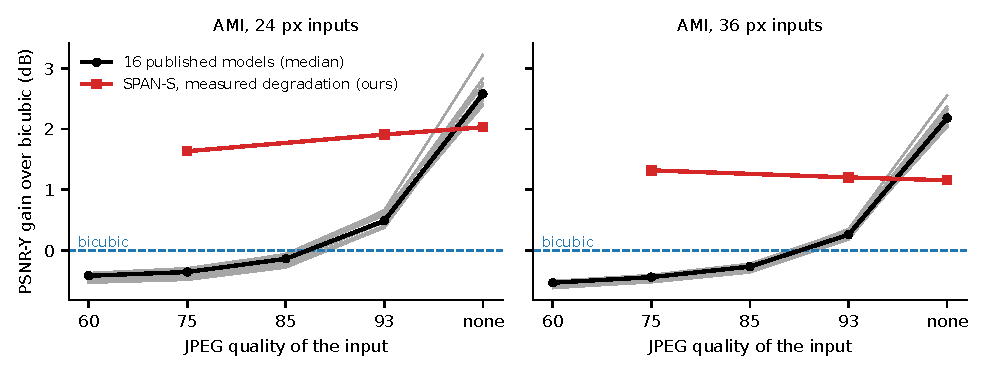
\includegraphics[width=\linewidth]{figures/fig_jpeg_sweep.pdf}
\caption{PSNR gain over bicubic interpolation as a function of the JPEG quality of the input, on AMI. Grey: each of the \NPub{} published fidelity-oriented models (\NAmiAllImg{} images); black: their median. Red: SPAN fine-tuned with the measured degradation (Section~\ref{sec:method}; each model on the test subjects of its fold).}
\label{fig:sweep}
\end{figure}

\subsection{The effect is not specific to one dataset or one input size}
Table~\ref{tab:generality} repeats the comparison at the three input sizes of AMI and on the two in-the-wild datasets. At quality 75, all \NPub{} models are significantly below bicubic at every input size of AMI and on AWEx at both sizes. On EarVN1.0 the mean gain is negative for \EarvnQLowBelow{} of the \NPub{} models and significantly so for \EarvnQLowSig{}; the remaining models are statistically tied with interpolation. At quality 93 no model is below bicubic on any dataset. Under the measured degradation, which mixes the two levels, the published models are within \WildEstGainMin{} to \WildEstGainMax{}~dB of bicubic on the in-the-wild sets, compared with a gain of \WildCleanGainMin{} to \WildCleanGainMax{}~dB on clean inputs. We therefore state the finding as follows: \emph{on small ear images, bicubic-trained SR models lose their fidelity advantage over interpolation under realistic compression, and fall below it from a JPEG quality of about 85 downwards}. The deficit does not grow as the input shrinks (SPAN: \SpanQLowGapS{}, \SpanQLowGapM{} and \SpanQLowGapL{}~dB at 24, 36 and 48 pixels); it is a property of the compression, present at every size we test.

\begin{table}[t]
\centering
\caption{Median PSNR gain over bicubic interpolation of the \NPub{} published fidelity-oriented models (dB), by dataset, input size and input degradation. In parentheses: number of models whose mean gain is negative / number whose 95\% confidence interval lies entirely below zero. ``--'': not evaluated.}
\label{tab:generality}
\resizebox{\linewidth}{!}{%
\begin{tabular}{@{}lrrccccc@{}}
\toprule
Dataset & Input (px) & Images & Clean & JPEG 93 & JPEG 85 & JPEG 75 & Measured \\
\midrule
\tabinput{generated/tab_generality}
\bottomrule
\end{tabular}}
\end{table}

\subsection{Ears, small inputs, or compression? A control on natural images}
\label{sec:natural}
Three things distinguish our benchmark from the protocol under which these models were trained: the content (ears), the input size (a few dozen pixels) and the compression. To separate them we evaluate the same \NPub{} models on natural images: the \NatN{} validation images of DIV2K~\cite{agustsson2017div2k}, each downsized to inputs of 24 to \NatLargePx{} pixels and degraded with the same JPEG levels (Table~\ref{tab:natural}). No model is trained or added for this control. The result separates the three factors. \emph{Input size does not move the crossover.} At JPEG quality 75 every model remains above bicubic interpolation on natural images at every input size, with a median gain of \NatSQLowMed{}~dB at 36-pixel inputs and \NatLQLowMed{}~dB at \NatLargePx{}-pixel inputs; at quality 60 every model is below it at every size (\NatSQVLowMed{} and \NatLQVLowMed{}~dB). \emph{Content does.} For natural images the crossover lies between quality 75 and 60; for ear images it lies between 93 and 85. \emph{The collapse of architectural differences is general.} On natural images the \NPub{} models span \NatSpreadCleanS{}~dB on clean 36-pixel inputs and \NatSpreadQLowS{}~dB at quality 75, as they do on ears.

\paragraph{One quantity accounts for both observations} Let $E_i$ be the mean squared error of bicubic interpolation of the clean input, and $E_c$ the additional error of bicubic interpolation when the input is compressed. Figure~\ref{fig:ratio} plots the median gain of the \NPub{} models against the ratio $E_c/E_i$ for all \RatioCells{} combinations of dataset, input size and JPEG quality in the \RatioSets{} datasets (inputs of \RatioPxMin{} to \RatioPxMax{} pixels, quality 60 to 93). In every combination with $E_c/E_i\le\RatioMaxAbove$ all \NPub{} models are above bicubic interpolation; in every combination with $E_c/E_i\ge\RatioMinBelow$ all of them are below it, except on EarVN1.0 at quality 75, where \EarvnQLowBelow{} are. The rank correlation between the ratio and the gain is \RatioSpearman{}. The rationale is simple: an SR network reduces the interpolation error and amplifies the compression error, so it can win only while the second is small relative to the first. Ear images are smooth. Bicubic interpolation of a clean 36-pixel input reaches \BicCleanPsnr{}~dB on AMI against \NatSBicClean{}~dB on DIV2K, so $E_i$ is small and a given JPEG quality contributes a far larger share of the error: at quality 75 the ratio is \RatioAmiQLow{} for AMI and \RatioDivQLow{} for DIV2K, and AMI at quality 93 has the same ratio as DIV2K at quality 60 (\RatioAmiQHigh{} and \RatioDivQVLow{}). What is specific to ear images is therefore not the phenomenon but its location: the compression levels that real small ear images carry lie beyond the threshold, whereas for natural images at the same levels they do not.

The threshold of about \RatioThresh{} is empirical. It is observed for bicubic-trained $\times4$ models and JPEG compression only, and the two combinations closest to it lie on opposite sides at almost the same ratio with gains that differ in size, so the gain is not a function of the ratio alone.

\begin{figure}[t]
\centering
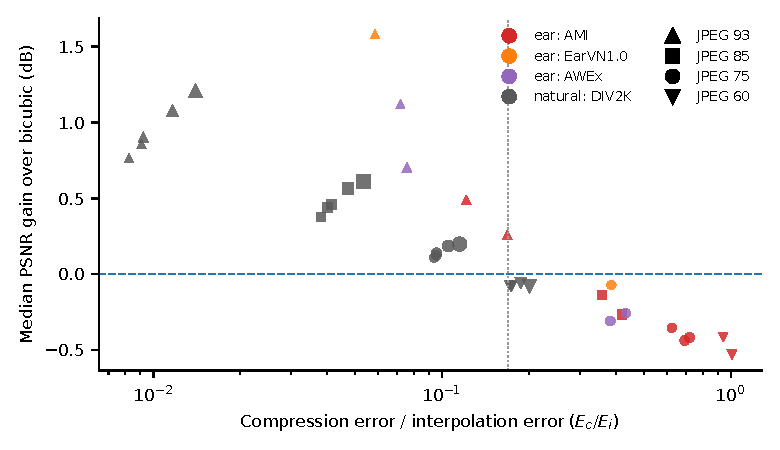
\includegraphics[width=0.8\linewidth]{figures/fig_ratio.pdf}
\caption{Median PSNR gain of the \NPub{} published models over bicubic interpolation against the ratio of compression error to interpolation error, for every dataset, input size (marker size) and JPEG quality. The dotted line marks the empirical threshold.}
\label{fig:ratio}
\end{figure}

\begin{table}[t]
\centering
\caption{Natural images against ear images: median PSNR gain over bicubic interpolation of the \NPub{} published models (dB) by input size and input degradation. In parentheses: number of models with negative mean gain / number significantly below zero.}
\label{tab:natural}
\resizebox{\linewidth}{!}{%
\begin{tabular}{@{}lrrccccc@{}}
\toprule
Images & Input (px) & Images & Clean & JPEG 93 & JPEG 85 & JPEG 75 & JPEG 60 \\
\midrule
\tabinput{generated/tab_natural}
\bottomrule
\end{tabular}}
\end{table}

\subsection{Fidelity and perceptual metrics disagree}
At quality 75, \LpipsQLowBetter{} of the \NPub{} models still have a lower LPIPS than bicubic interpolation (for SPAN, \SpanQLowLpips{} against \BicQLowLpips{}). The outputs look sharper while being further from the ground truth. This matters for how the finding is worded, and for applications: where the enlarged image is evidence, or the input of a recognition system, sharper but less faithful is not obviously an improvement. The perceptual models make the trade explicit. BSRGAN reaches an LPIPS of \BsrganQLowLpips{} at quality 75, the best of all models, at a PSNR \BsrganQLowGap{}~dB below bicubic interpolation and at \LatRatio{} times the latency of SPAN.

\subsection{Architecture is not the bottleneck}
\label{sec:capacity}
On clean inputs the \NPub{} models span \SpreadClean{}~dB and capacity pays: the \ParamsRrdb{}M-parameter RRDB exceeds the \ParamsSpan{}M-parameter SPAN by \RrdbVsSpanCleanL{}, \RrdbVsSpanCleanM{} and \RrdbVsSpanCleanS{}~dB at 48, 36 and 24-pixel inputs, more as the input shrinks. Under JPEG 75 the same models span only \SpreadQLow{}~dB, RRDB is \RrdbVsSpanQLowM{}~dB from SPAN, and the ranking of the models is unrelated to their ranking on clean inputs (Kendall's $\tau=\TauRank$ between the two orderings by mean PSNR). No choice among the published architectures recovers the lost fidelity. Section~\ref{sec:experiments} shows that a change of training degradation on a single architecture does.

\section{Training with a measured degradation}
\label{sec:method}
We keep a published real-time backbone and change its fine-tuning in two respects: the degradation applied to the training images (Section~\ref{sec:measured}) and the photometric range of the training data (Section~\ref{sec:stable}).

\subsection{Degradation of real small ear images}
\label{sec:measured}
We use the images of the \RoleFit{} EarVN1.0 subjects reserved for this purpose, which comprise \FitSmall{} real small images (short side 24 to 48 pixels) and \FitLarge{} large images. Three quantities are estimated.

\paragraph{Compression level} A JPEG file stores its quantisation tables, from which the quality setting of a standard encoder can be recovered. In the real small images the distribution is bimodal: \QLowShare{}\% of the images are at quality 75 and \QHighShare{}\% at quality 93, with the remainder at neighbouring values. We use this empirical distribution.

\paragraph{Noise} We apply the estimator of Immerk{\ae}r~\cite{immerkaer1996noise} to each real small image and use the 5th to 95th percentile range, \NoiseLo{} to \NoiseHi{} on the 8-bit scale. Because the images are already compressed, this range underestimates the noise before compression.

\paragraph{Blur} A blur kernel is difficult to identify from a compressed image of a few dozen pixels. We select, from a set of candidate ranges for the width of an isotropic Gaussian, the range for which the sharpness statistics (Laplacian energy normalised by variance) of large images degraded with the full pipeline are closest to those of the real small images in Kolmogorov--Smirnov distance. The selected range is $\sigma\in[\BlurLo,\BlurHi]$ input pixels, which corresponds to a small amount of blur.

The resulting pipeline consists of Gaussian blur, bicubic downsampling, Gaussian noise and JPEG compression, with parameters drawn independently for each training sample. The generic pipeline of Section~\ref{sec:degradations} has the same structure with wider parameter ranges.

\paragraph{Comparison with real images} To assess how close the simulated images are to real ones, we train a small convolutional classifier to separate $16\times16$ patches of real small ear images from patches of simulated images, which are generated from large images of the same subjects and brought to the same size distribution. Subjects are split between training and testing (\RealTrainSubj{} and \RealTestSubj{} subjects of the classifier group), and the experiment is repeated with three seeds. Table~\ref{tab:realism} gives the balanced accuracy, where 50\% means that the classifier does not separate simulated from real images. The classifier separates bicubic downsampling (\RealBic{}\%) and the generic pipeline (\RealGen{}\%) from real images with similar accuracy, so by this test the generic pipeline is not closer to the real data than bicubic downsampling. The measured pipeline gives \RealEst{}\%. Bicubic downsampling followed by JPEG at quality 75 gives \RealJpg{}\%, which is not significantly different from the measured pipeline. By this test, compression is the main factor that makes the simulated images similar to real ones. We return to this point in Section~\ref{sec:ablation}.

\begin{table}[t]
\centering
\caption{Balanced accuracy (\%) of a classifier trained to separate real small ear images from simulated ones, on held-out subjects. Closer to 50\% means more realistic. Intervals are 95\% bootstrap intervals.}
\label{tab:realism}
\small
\begin{tabular}{@{}lcc@{}}
\toprule
Simulated with & Accuracy & 95\% CI \\
\midrule
\tabinput{generated/tab_realism}
\bottomrule
\end{tabular}
\end{table}

\subsection{Stability of fine-tuning}
\label{sec:stable}
Our first models were fine-tuned on AMI alone. Their validation PSNR on AMI improved, but on EarVN1.0 the SPAN model fine-tuned with bicubic downsampling reached \CollapsePsnr{}~dB on clean inputs, compared with \CollapsePub{}~dB for the published weights it was initialised from and \CollapseBic{}~dB for bicubic interpolation. \CollapseBroken{} of the \NEarvnImg{} outputs were below 20~dB and contained high-amplitude noise. The failures occurred mainly on images with bright regions. AMI was acquired under uniform indoor lighting and contains few such images. Our inspection of the network suggests that, after fine-tuning, the activations of the attention blocks grow from block to block for inputs brighter than the training images. Validation on held-out AMI subjects did not reveal the problem.

Two changes prevented this failure in our experiments. The first is a photometric augmentation: with probability 0.75 the ground-truth patch is multiplied by a random gain (log-uniform in $[0.7, 2.2]$), raised to a random gamma ($[0.7,1.4]$) and scaled per channel ($[0.9,1.1]$) before the degradation is applied. The second is the addition of in-the-wild training images: 30\% of the training samples are drawn from the large images of the EarVN1.0 training subjects. We also add a stress test to each training run. The validation images are brightened by factors of 1.4 and 1.8, and a run is marked as unstable if any output is more than 10~dB below bicubic interpolation or if the margin of the model over bicubic interpolation decreases by more than 1.5~dB. All \NRuns{} runs reported in this paper pass this test (largest decrease \StressMaxDrop{}~dB). Table~\ref{tab:stability} shows the effect of the two changes.

\begin{table}[t]
\centering
\caption{Effect of the fine-tuning recipe on clean inputs (PSNR-Y, dB): SPAN fine-tuned with bicubic downsampling. $^\dagger$One run, excluded from all other results.}
\label{tab:stability}
\small
\begin{tabular}{@{}lcccc@{}}
\toprule
 & AMI & EarVN1.0 & AWEx & AWEx \\
 & 36 px & 24 px & 24 px & 36 px \\
\midrule
\tabinput{generated/tab_stability}
\bottomrule
\end{tabular}
\end{table}

\subsection{Training details}
We fine-tune from the published weights for 20{,}000 iterations with the $L_1$ loss, Adam~\cite{kingma2015adam} with an initial learning rate of $2\times10^{-4}$ and cosine decay, batches of 64 input patches of $24\times24$ pixels, and an exponential moving average of the weights (decay 0.999). Each AMI training image is first resized so that its short side is drawn at random between 96 and 192 pixels, so that one model covers the three benchmark sizes. The checkpoint with the highest PSNR on the validation subjects of the fold is kept. The random seed of a run equals its fold index. One run takes about half an hour on an RTX~3080. We apply the procedure to two backbones from different architecture families: SPAN with 48 channels~\cite{wan2024span} and DISP, an entry of the NTIRE 2026 challenge~\cite{ren2026ntire}.

\section{Experiments}
\label{sec:experiments}

\subsection{Setup}
For each backbone and each fold we fine-tune one model per training degradation: \emph{bicubic}, \emph{generic}, \emph{bicubic + JPEG 75} and \emph{measured}. All use the recipe of Section~\ref{sec:stable} and differ in nothing else, so differences between them are attributable to the degradation. Together with the two ablation runs per fold of Table~\ref{tab:stability} and the two JPEG-only variants of Section~\ref{sec:ablation} this gives \NRuns{} runs over the \NFolds{} folds. Models are compared with bicubic interpolation and with the published weights of the same backbone on four cells: AMI with 36-pixel inputs (\NAmiImg{} images of \NAmiSubj{} subjects), EarVN1.0 with 24-pixel inputs (\NEarvnImg{} images, \NEarvnSubj{} subjects) and AWEx with 24 and 36-pixel inputs (\NAwexSImg{} and \NAwexMImg{} images).

\subsection{The training degradation decides}
Table~\ref{tab:matrix} crosses the training degradation with the degradation of the test input, for SPAN on AMI. Three observations follow. First, fine-tuning on ear images with bicubic downsampling improves the clean column and nothing else: under compression the fine-tuned model is as far below bicubic interpolation as the published weights. Domain data without the right degradation does not help. Second, the generic pipeline yields a model that is below bicubic interpolation on clean inputs on all four cells (by \GenVsBicCleanMin{} to \GenVsBicCleanMax{}~dB) and between \GenVsBicEstMin{} and \GenVsBicEstMax{}~dB of it on inputs degraded with the measured pipeline; it is the best choice only on inputs produced by the generic pipeline itself, which the classifier of Section~\ref{sec:measured} shows to be unlike real small ear images. Third, on JPEG~75 inputs the measured degradation recovers \DegEffMin{} to \DegEffMax{}~dB over bicubic training across the four cells, and the fixed JPEG~75 degradation \JpgEffMin{} to \JpgEffMax{}~dB. This is an order of magnitude more than the \SpreadQLow{}~dB that separates the \NPub{} published architectures under the same inputs (Section~\ref{sec:capacity}).

\begin{table}[t]
\centering
\caption{PSNR-Y (dB) of SPAN on AMI (36-pixel inputs) by training degradation (rows) and test input (columns). Best fine-tuned or published model per column in bold.}
\label{tab:matrix}
\resizebox{\linewidth}{!}{%
\begin{tabular}{@{}lccccc@{}}
\toprule
 & \multicolumn{5}{c}{Test input} \\
\cmidrule(l){2-6}
Training degradation & Clean & JPEG 93 & JPEG 75 & Measured & Generic \\
\midrule
\tabinput{generated/tab_matrix}
\bottomrule
\end{tabular}}
\end{table}

\subsection{Main result}
Table~\ref{tab:main} gives the paired differences between SPAN fine-tuned with the measured degradation and each reference, on inputs degraded with the measured pipeline. The model exceeds bicubic interpolation by \EstVsBicMin{} to \EstVsBicMax{}~dB, the published weights by \EstVsPubMin{} to \EstVsPubMax{}~dB and the generic pipeline by \EstVsGenMin{} to \EstVsGenMax{}~dB; no confidence interval contains zero. LPIPS improves as well, by \EstLpipsVsBicMin{} to \EstLpipsVsBicMax{} over bicubic interpolation and by \EstLpipsVsGenMin{} to \EstLpipsVsGenMax{} over the generic pipeline. The result holds in each fold separately, including the two held-out folds (measured minus generic on AMI: \EstVsGenFoldMin{} to \EstVsGenFoldMax{}~dB across folds), on inputs compressed at a single quality (\EstVsBicQLowMin{} to \EstVsBicQLowMax{}~dB over bicubic at quality 75 and \EstVsBicQHighMin{} to \EstVsBicQHighMax{}~dB at quality 93), and for the second backbone: DISP fine-tuned with the measured degradation exceeds bicubic interpolation by \DispEstVsBicMin{} to \DispEstVsBicMax{}~dB and its generic counterpart by \DispEstVsGenMin{} to \DispEstVsGenMax{}~dB. The gain is larger for smaller inputs (Figure~\ref{fig:size}): \EstVsBicAmiS{}, \EstVsBicAmiM{} and \EstVsBicAmiL{}~dB over bicubic at 24, 36 and 48 pixels on AMI.

\begin{table}[t]
\centering
\caption{SPAN fine-tuned with the measured degradation \emph{minus} each reference, on inputs degraded with the measured pipeline. Paired differences with 95\% confidence intervals (bootstrap over subjects).}
\label{tab:main}
\resizebox{\linewidth}{!}{%
\begin{tabular}{@{}lcccc@{}}
\toprule
Ours minus & AMI, 36 px & EarVN1.0, 24 px & AWEx, 24 px & AWEx, 36 px \\
\midrule
\tabinput{generated/tab_main}
\bottomrule
\end{tabular}}
\end{table}

\begin{figure}[t]
\centering
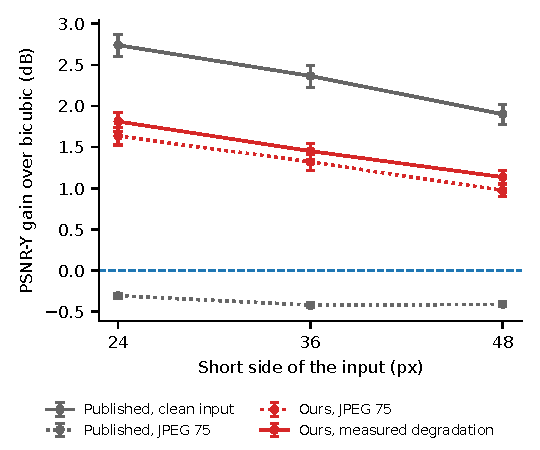
\includegraphics[width=0.55\linewidth]{figures/fig_size.pdf}
\caption{PSNR gain over bicubic interpolation by input size on AMI, for the published SPAN weights and for SPAN fine-tuned with the measured degradation. Bars: 95\% confidence intervals.}
\label{fig:size}
\end{figure}

\paragraph{The price} The model is specialised to compressed inputs. On clean inputs it is \EstVsPubCleanMin{} to \EstVsPubCleanMax{}~dB below the published weights, while remaining above bicubic interpolation (Table~\ref{tab:matrix}). No single model is best for every input. Since real small ear images are compressed, we regard the trade as the right one for this domain, and report the clean column so that the reader can judge.

\subsection{What part of the measured degradation matters?}
\label{sec:ablation}
The realism classifier could not distinguish the measured degradation from bicubic downsampling followed by JPEG at quality 75. Table~\ref{tab:levels} asks the same question of the trained models. Against a model trained with the fixed quality 75, the measured degradation is better by \EstVsJpgHighMin{} to \EstVsJpgHighMax{}~dB on quality-93 inputs and by \EstVsJpgMin{} to \EstVsJpgMax{}~dB on the measured mixture, and worse by \EstVsJpgLowMin{} to \EstVsJpgLowMax{}~dB on quality-75 inputs, on which the fixed model is trained exactly. Training on the measured distribution of compression levels thus buys robustness across the levels that occur in practice for a negligible loss at any one of them.

\begin{table}[t]
\centering
\caption{Measured degradation \emph{minus} fixed JPEG~75, same backbone, by test input (PSNR-Y, dB; 95\% confidence intervals).}
\label{tab:levels}
\resizebox{\linewidth}{!}{%
\begin{tabular}{@{}llcccc@{}}
\toprule
Backbone & Test input & AMI, 36 px & EarVN1.0, 24 px & AWEx, 24 px & AWEx, 36 px \\
\midrule
\tabinput{generated/tab_levels}
\bottomrule
\end{tabular}}
\end{table}

To separate the contribution of the compression levels from that of the measured noise and blur, we train two further models: one with bicubic downsampling followed by JPEG at the measured distribution of levels, without noise or blur, and one with JPEG quality drawn uniformly from 60 to 95, which uses nothing measured from the data (Table~\ref{tab:ablation} and the corresponding rows of Table~\ref{tab:matrix}). On inputs degraded with the full measured pipeline, the measured model is ahead of the levels-only model by \EstVsMixMin{} to \EstVsMixMax{}~dB. On inputs with the same compression levels but without noise and blur the order reverses, the levels-only model being ahead by \MixVsEstOnMixMin{} to \MixVsEstOnMixMax{}~dB; it is also ahead at quality 93 (\MixVsEstHighMin{} to \MixVsEstHighMax{}~dB) and on clean inputs (\MixVsEstCleanMin{} to \MixVsEstCleanMax{}~dB). Each model is best on the inputs that match its own training, so synthesised inputs cannot decide whether the measured noise and blur are worth having. Real images can, and Section~\ref{sec:recog} finds no difference. The levels-only and the uniform-level models differ by \MixVsUniMin{} to \MixVsUniMax{}~dB on measured inputs: once the range of levels is covered, their exact distribution does not matter.

We conclude that the essential ingredient is JPEG compression over the range of quality levels found in the target images, here roughly 70 to 95. Measuring the degradation serves to identify that range; estimating noise and blur is not required. We keep the measured degradation as the reference model in all tables because it was fixed before these comparisons were run.

\begin{table}[t]
\centering
\caption{Separating compression levels from noise and blur: SPAN fine-tuned with the measured degradation \emph{minus} two JPEG-only variants (PSNR-Y, dB; 95\% confidence intervals).}
\label{tab:ablation}
\resizebox{\linewidth}{!}{%
\begin{tabular}{@{}llcccc@{}}
\toprule
Comparison & Test input & AMI, 36 px & EarVN1.0, 24 px & AWEx, 24 px & AWEx, 36 px \\
\midrule
\tabinput{generated/tab_ablation}
\bottomrule
\end{tabular}}
\end{table}

\subsection{Real small ear images: identification}
\label{sec:recog}
All results above use inputs synthesised from larger images, because real small images have no ground truth. Identity labels offer an objective measure that needs none. We take the subjects of EarVN1.0 that were used neither for SR training nor for any fitting (the test and reserved groups). For each subject, half of the large images (short side at least 96 pixels) are enrolled and their embeddings averaged into a template; \RecEnrolled{} subjects are enrolled with \RecGallery{} images. The probes are the \RecProbes{} \emph{real} small images (short side 24 to 48 pixels) of the \RecSubj{} enrolled subjects that have any. Each probe is enlarged $\times4$ by the method under test and resized to the input size of the recogniser by one fixed operation. The recogniser is a ResNet-18~\cite{he2016resnet} with a cosine-margin loss~\cite{wang2018cosface}, trained only on large images of \RecTrainSubj{} other subjects (\RecTrainImg{} images); it never sees a small or an upscaled image, so it does not favour the look of any upscaling method. As a control we repeat the experiment with frozen ImageNet features that have never seen an ear.

Table~\ref{tab:recog} reports rank-1 identification and equal error rate (EER). With large probes the recogniser reaches a rank-1 rate of \RecRankRef{}\% (EER \RecEerRef{}\%), which bounds what can be expected of small ones; on held-out images of its training subjects its accuracy is \RecValAcc{}\%. With real small probes and bicubic upscaling the rate is \RecRankBic{}\%. The methods fall into three groups.

\emph{Bicubic-trained models do not help.} The published SPAN weights reach \RecRankPub{}\% (\RecPubVsBic{} percentage points relative to bicubic upscaling), and SPAN fine-tuned on ear images with bicubic downsampling \RecRankBict{}\% (\RecBictVsBic{}).

\emph{Every compression-aware model nearly doubles the rate.} SPAN with the measured degradation reaches \RecRankEst{}\%, a paired gain of \RecEstVsBic{} points over bicubic upscaling and \RecEstVsPub{} over the published weights, and lowers the EER from \RecEerBic{}\% to \RecEerEst{}\% (\RecEerEstVsBic{}). The second backbone behaves alike (DISP: \RecRankDispEst{}\%, \RecDispEstVsBic{} over bicubic). Within the group the differences are small. The fixed JPEG~75 and uniform-level variants are indistinguishable from our model (\RecJpgVsEst{} and \RecUniVsEst{} points); the levels-only variant and the generic pipeline are about one point lower (\RecMixVsEst{} and \RecGenVsEst{}).

\emph{Large GAN-trained models are not significantly better.} BSRGAN and Real-ESRGAN reach \RecRankBsrgan{}\% and \RecRankRealesrgan{}\% (\RecBsrganVsEst{} points for BSRGAN relative to our model), at \LatRatio{} times the latency.

The control recogniser, which has never seen an ear, gives much lower rates and the same ordering: \RecCtlRankBic{}\% with bicubic upscaling, \RecCtlRankPub{}\% with the published weights and \RecCtlRankEst{}\% with our model (\RecCtlEstVsBic{} over bicubic).

\begin{table}[t]
\centering
\caption{Identification of real small ear images (short side 24 to 48 pixels) after $\times4$ upscaling. Rank-1 rate with 95\% confidence interval and equal error rate, in \%, for an ear recogniser and for frozen ImageNet features. Fine-tuned rows average the models of the folds.}
\label{tab:recog}
\resizebox{\linewidth}{!}{%
\begin{tabular}{@{}lcccc@{}}
\toprule
 & \multicolumn{2}{c}{Ear recogniser (ResNet-18)} & \multicolumn{2}{c}{ImageNet features (ResNet-50)} \\
\cmidrule(lr){2-3}\cmidrule(l){4-5}
Upscaling & Rank-1 & EER & Rank-1 & EER \\
\midrule
\tabinput{generated/tab_recog}
\bottomrule
\end{tabular}}
\end{table}

\paragraph{By compression level of the probe} The quality setting of each real probe can be read from its file, which allows a direct test of the threshold found on synthesised inputs in Section~\ref{sec:analysis}. Table~\ref{tab:recogquality} splits the probes into those stored at JPEG quality 70 to 80 (\RecQLowN{} probes of \RecQLowSubj{} subjects) and those stored at quality 90 or above (\RecQHighN{} probes of \RecQHighSubj{} subjects). For the heavily compressed probes the published SPAN weights change the rank-1 rate by \RecQLowPub{} points relative to bicubic upscaling; for the lightly compressed ones by \RecQHighPub{}. The compression-aware model gains \RecQLowEst{} and \RecQHighEst{} points. The pattern predicted from synthesised inputs, a bicubic-trained model that is useful at quality 93 and not at quality 75, is thus observed on real images through an independent measure. The table also locates the advantage of the GAN-trained models: BSRGAN gains \RecQHighBsrgan{} points on the lightly compressed probes and \RecQLowBsrgan{} on the heavily compressed ones. The two groups contain largely different subjects, so the comparison is between methods within a group, not between groups.

\begin{table}[t]
\centering
\caption{Rank-1 identification (\%) of real small ear images by the JPEG quality stored in the probe file, and paired difference from bicubic upscaling in percentage points with 95\% confidence interval (EarVN1.0, ear recogniser).}
\label{tab:recogquality}
\resizebox{\linewidth}{!}{%
\begin{tabular}{@{}lcccc@{}}
\toprule
 & \multicolumn{2}{c}{Quality 70--80} & \multicolumn{2}{c}{Quality $\geq$ 90} \\
\cmidrule(lr){2-3}\cmidrule(l){4-5}
Upscaling & Rank-1 & vs.\ bicubic & Rank-1 & vs.\ bicubic \\
\midrule
\tabinput{generated/tab_recog_quality}
\bottomrule
\end{tabular}}
\end{table}

\paragraph{A second dataset and a second recogniser} To test whether these results depend on the recogniser or on the dataset, we repeat the experiment with a second ear recogniser, a ResNet-50 trained on the same data (\RecRfValAcc{}\% accuracy on held-out images of its training subjects), and on AWEx, which was used for no training of any kind (\RecAwexEnrolled{} subjects enrolled, \RecAwexProbes{} real small probes of \RecAwexSubj{} subjects, same protocol). Table~\ref{tab:recogrobust} gives the paired differences from bicubic upscaling.

The second recogniser confirms the result on EarVN1.0: the rank-1 rate rises from \RecEarvnRfRankBic{}\% with bicubic upscaling to \RecEarvnRfRankEst{}\% with our model (\RecEarvnRfEstVsBic{} points), against \RecEarvnRfPubVsBic{} for the published weights. With this recogniser the generic pipeline is significantly below our model (\RecEarvnRfGenVsEst{} points).

AWEx behaves differently. No upscaling method changes the rank-1 rate significantly there, with either recogniser: our model by \RecAwexReEstVsBic{} and \RecAwexRfEstVsBic{} points, the published weights by \RecAwexRePubVsBic{} and \RecAwexRfPubVsBic{}, BSRGAN by \RecAwexReBsrganVsBic{} and \RecAwexRfBsrganVsBic{}. \emph{The gain observed on EarVN1.0 is not replicated on AWEx.}

\paragraph{When does upscaling help identification?} The two datasets differ in two respects, each of which bounds what an upscaling step can contribute. We examined them after seeing the AWEx result, and report them as conditions suggested by the data, not as an established explanation.

\emph{Compression.} The small AWEx images carry no JPEG block structure. The ratio of pixel differences across $8\times8$ block boundaries to differences inside blocks has a median of \BlockAwex{} for the AWEx probes, against \BlockEarvnLow{} for the EarVN1.0 probes stored at quality 70 to 80 and \BlockEarvnHigh{} for those at quality 90 or above; AWEx is distributed as PNG and its compression history is unknown. A compression-aware model has no blocking to remove there.

\emph{Headroom.} Upscaling can at best give back what low resolution took from the recogniser. We call \emph{headroom} the difference between the rank-1 rate of large probes and that of bicubically upscaled small probes. On EarVN1.0 it is large (\RecRankRef{}\% against \RecRankBic{}\% with the ResNet-18 recogniser); on AWEx, where a subject has a median of \RecAwexGalMed{} enrolled images against \RecEarvnGalMed{} on EarVN1.0, it is absent (\RecAwexReRankRef{}\% against \RecAwexReRankBic{}\%). Within EarVN1.0 the gain of our model follows the headroom of the subject: among the \HeadEarvnReSubj{} subjects with at least five small probes, the half with less headroom (\HeadEarvnReLowRoom{} points on average) gains \HeadEarvnReLowGain{} points and the half with more (\HeadEarvnReHighRoom{}) gains \HeadEarvnReHighGain{}; with the ResNet-50 recogniser the two halves gain \HeadEarvnRfLowGain{} and \HeadEarvnRfHighGain{}. The rank correlation between headroom and gain is positive but does not reach significance at this number of subjects (Spearman $\rho=\HeadEarvnReRho$, $p=\HeadEarvnReP$, and $\rho=\HeadEarvnRfRho$, $p=\HeadEarvnRfP$). Headroom alone is not sufficient: the AWEx subjects that do have it (\HeadAwexReHighRoom{} points in the upper half) gain \HeadAwexReHighGain{} and \HeadAwexRfHighGain{} points with the two recognisers, although these per-subject figures rest on a median of two probes.

In our data, then, upscaling improves identification where the probes are compressed \emph{and} the recogniser loses accuracy at low resolution. EarVN1.0 meets both conditions and AWEx neither, so the two datasets cannot separate them; the split by file quality and the split by headroom within EarVN1.0 are the only within-dataset evidence for each.

\begin{table}[t]
\centering
\caption{Robustness of the identification result: paired difference in rank-1 rate from bicubic upscaling (percentage points, 95\% confidence interval), on two datasets and with two ear recognisers. The first two rows give absolute rank-1 rates.}
\label{tab:recogrobust}
\resizebox{\linewidth}{!}{%
\begin{tabular}{@{}lcccc@{}}
\toprule
 & \multicolumn{2}{c}{EarVN1.0} & \multicolumn{2}{c}{AWEx} \\
\cmidrule(lr){2-3}\cmidrule(l){4-5}
Upscaling & ResNet-18 & ResNet-50 & ResNet-18 & ResNet-50 \\
\midrule
\tabinput{generated/tab_recog_robust}
\bottomrule
\end{tabular}}
\end{table}

Three conclusions follow. First, on real small ear images that are JPEG-compressed, the finding of Section~\ref{sec:analysis} carries over: SR trained with bicubic downsampling gives no identification benefit, with or without fine-tuning on ear data, and compression-aware training does, with two recognisers and a control. Second, the choice among compression-only degradations makes no measurable difference to identification, which settles the question left open in Section~\ref{sec:ablation}; the generic pipeline is slightly but significantly worse, in addition to its lower fidelity (Table~\ref{tab:main}). Third, the benefit is conditional: it appears where the probes are compressed and the recogniser has headroom between large and small images, it varies with the quality stored in the probe files and with the headroom of the subject, and it is absent on AWEx, where neither condition holds. We therefore do not claim that SR improves ear identification in general; we claim to have identified when it does. Figure~\ref{fig:qualitative} shows examples.


\begin{figure}[t]
\centering
\tabinput{generated/fig_qualitative}
\caption{Real small ear images from EarVN1.0 (short side 24 to 48 pixels) enlarged $\times4$. The published weights sharpen the compression blocks; the compression-aware models remove them. \todo{select examples from several subjects; check the image rights for publication.}}
\label{fig:qualitative}
\end{figure}

\subsection{Real small ear images: viewer preference}
\todo{viewer study on real small images of the reserved subjects: pairs (ours vs.\ bicubic, ours vs.\ published weights, ours vs.\ generic), number of viewers, preference rate with confidence interval. Tools: \texttt{evaluate.py --save-sr}, \texttt{viewer\_study.py}.}

\subsection{Efficiency}
\label{sec:efficiency}
The method changes the weights of the backbone and nothing else, so its cost is that of the backbone. We take real time to mean a median latency of at most 33~ms (30 frames per second) for one $48\times68$ input, the largest input size considered here. On a desktop GPU (RTX~3080, 32-bit precision) SPAN with 48 channels (\ParamsSpan{}M parameters) needs \LatSpan{}~ms and DISP \LatDisp{}~ms, against \LatBsrgan{}~ms for BSRGAN (Table~\ref{tab:published}).

To test the claim on consumer hardware we convert the models to Core ML with 16-bit weights and measure them on an \PhoneName{} (\PhoneChip{}, iOS \PhoneOs{}), a phone released in 2020, with the performance tool of Xcode, which reports the median prediction time on the device. Table~\ref{tab:latencyios} gives the result with computation restricted to the CPU and with all compute units (CPU, GPU and neural engine) allowed. SPAN runs in \LatPhoneSpanCpu{}~ms on the CPU alone and \LatPhoneSpanAll{}~ms with all units; DISP in \LatPhoneDispCpu{} and \LatPhoneDispAll{}~ms; BSRGAN in \LatPhoneBsrganCpu{} and \LatPhoneBsrganAll{}~ms. \todo{state which models meet the 33~ms threshold once the measurements exist; if SPAN does not, change ``Real-Time'' in the title. The tool reports medians only; no 95th percentile is available.} The converted models reproduce the PyTorch outputs to within 16-bit rounding (PSNR between the two outputs: \CoremlPsnrSpan{}~dB for SPAN and \CoremlPsnrDisp{}~dB for DISP).

\begin{table}[t]
\centering
\caption{Median latency (ms) for one $48\times68$ input at $\times4$: desktop GPU (RTX~3080, PyTorch, 32-bit) and smartphone (\PhoneName{}, Core ML, 16-bit).}
\label{tab:latencyios}
\small
\begin{tabular}{@{}lrccc@{}}
\toprule
 & Params & Desktop & \multicolumn{2}{c}{Smartphone} \\
\cmidrule(l){4-5}
Model & (K) & GPU & CPU only & All units \\
\midrule
\tabinput{generated/tab_latency_ios}
\bottomrule
\end{tabular}
\end{table}

\section{Discussion and limitations}
\label{sec:discussion}

\paragraph{What is new and what is not} That SR models trained on bicubic downsampling degrade on compressed inputs is known for natural images. What this study adds is a measurement in a regime and a domain where it had not been made: inputs of a few dozen pixels of a biometric trait, where the compression level at which published efficient models stop being useful (about quality 85) falls between the two levels that real images of the domain actually have; the observation that a generic real-world pipeline is not a remedy there; and the observation that, once the degradation is repaired, a \ParamsSpan{}M-parameter network suffices to exceed every published model we tested in fidelity, including one \ParamsRatio{} times larger.

\paragraph{Limits of the claim} (i) The model is better than the published fidelity-oriented models and than bicubic interpolation on compressed inputs, in fidelity and in LPIPS. It is not better on clean inputs, and large GAN-trained models keep a lower LPIPS at a much lower fidelity and a much higher cost. (ii) Most of the gain over a fixed-quality JPEG degradation is explained by the distribution of compression levels (Section~\ref{sec:ablation}); we do not claim that estimating noise and blur is necessary. (iii) Fidelity results rely on synthesised inputs. The in-the-wild datasets have ground truth only at the smallest sizes, and the evaluation on real small images is through identification and viewer preference, not fidelity. (iv) AMI was photographed indoors and has 100 subjects; each fold is trained with one seed, so the spread across folds stands in for the spread across seeds. (v) The realism classifier is evaluated on \RealTestSubj{} held-out subjects; an accuracy near 50\% shows that this classifier cannot separate the two sets, not that the distributions coincide. (vi) The blur of real small images is matched only through a sharpness statistic.

\paragraph{Practical guidance} For small ear images that have been through JPEG compression, a published efficient SR model should not be assumed to improve on interpolation. Fine-tuning on ear images is not sufficient if the degradation is left unchanged, and a generic real-world degradation is not a substitute for one that covers the compression levels of the target images. When the fine-tuning data come from a controlled acquisition, photometric augmentation and a brightness stress test should be part of the procedure.

\section{Conclusion}
On small ear images, published efficient SR models fall below bicubic interpolation in fidelity under the compression that real images of the domain carry, and no choice among sixteen architectures changes this. Repairing the training degradation does: a real-time network fine-tuned with a degradation measured from real small ear images, under a recipe that keeps fine-tuning stable outside the laboratory data, exceeds bicubic interpolation and the published models on three datasets at no additional cost. The benchmark, the measured degradation and the baselines are released so that architectures designed for such inputs can be compared against a model that is trained correctly.


\section*{Data and code availability}
All datasets used are public. The code, the subject-wise splits, the measured degradation parameters, the per-image result files behind every table and the trained weights will be released at \todo{repository URL}.

\bibliographystyle{elsarticle-num}
\bibliography{refs}
\end{document}
